% !TEX root = ../tex/8-1.tex
% 第8章：本文は青、補足は緑
\newcommand{\asmain}{%
    \setbeamercolor{frametitle}{fg=white,bg=main}%
    \setbeamercolor{structure}{fg=main}%
    \setbeamercolor{itemize item}{fg=main}%
    \setbeamercolor{itemize subitem}{fg=main}%
    \setbeamercolor{enumerate item}{fg=main}%
}
\newcommand{\assuppl}{%
    \setbeamercolor{frametitle}{fg=white,bg=examplecol}%
    \setbeamercolor{structure}{fg=examplecol}%
    \setbeamercolor{itemize item}{fg=examplecol}%
    \setbeamercolor{itemize subitem}{fg=examplecol}%
    \setbeamercolor{enumerate item}{fg=examplecol}%
}
\newcommand{\supplmark}{%
    \setlength{\fboxsep}{1.5pt}%
    \setlength{\fboxrule}{0.7pt}%
    \fbox{\textbf{補足}}%
}
\asmain


%=============================================
\begin{frame}{第7章から第8章へ}
    \begin{block}{ここまで（第7章・任意）}
        分布間翻訳とOT／SBのレンズで、\\
        「どう運ぶか」の最適性を整理した。
    \end{block}
    \begin{block}{ここから（第8章）}
        生成軌道を\textbf{ユーザ意図で操る}枠組みへ。\\
        逆時間スコア／PF-ODEに誘導方向$G_t$を足すのが基本形。
    \end{block}
\end{frame}
%=============================================
\asmain
\begin{frame}{この章の位置づけ}
    \begin{block}{中心の問い}
        無条件の生成軌道を、条件・嗜好に合わせて\\
        どのように\textbf{誘導（guidance）}できるか？
    \end{block}
    \begin{itemize}
        \item 粗から細への生成過程は、途中介入の余地を与える
        \item ベイズ分解が「無条件方向＋誘導方向」の加法構造を示す
        \item CG／CFG／学習不要誘導／嗜好整合が同じテンプレートに乗る
    \end{itemize}
\end{frame}
%=============================================
\asmain
\begin{frame}{8.1 の位置づけと学習目標}
    \begin{block}{この節の役割}
        制御可能生成の動機を置き、\\
        誘導の共通テンプレートと各手法の予告を行う序章
    \end{block}
    \begin{enumerate}
        \item ベイズ分解と誘導方向$G_t$、誘導付きPF-ODE（8.1.2--8.1.3）
        \item CG／CFG／学習不要／嗜好整合の役割分担
        \item 固定時刻の傾き密度と、誘導サンプラ周辺の違いに注意
    \end{enumerate}
\end{frame}
%=============================================
\section{動機：制御可能生成}
\asmain
\begin{frame}{区切り：動機：制御可能生成}
    \tableofcontents[currentsection]
\end{frame}
%=============================================
\asmain
\begin{frame}{粗から細への生成と介入}
    拡散の生成は粗$\to$細に進む：
    \begin{itemize}
        \item 各ステップでわずかにノイズを除き、構造と細部が現れる
        \item 時間依存の速度場（スコア）に\textbf{誘導項}を足せば、\\
        ユーザ意図に沿って軌道を曲げられる
    \end{itemize}
    \begin{exampleblock}{直感}
        「最終サンプルだけ」ではなく、\\
        軌道そのものを条件・属性へ寄せる。
    \end{exampleblock}
\end{frame}
%=============================================
\asmain
\begin{frame}{図8.1：誘導付き拡散サンプリング}
    \centering
    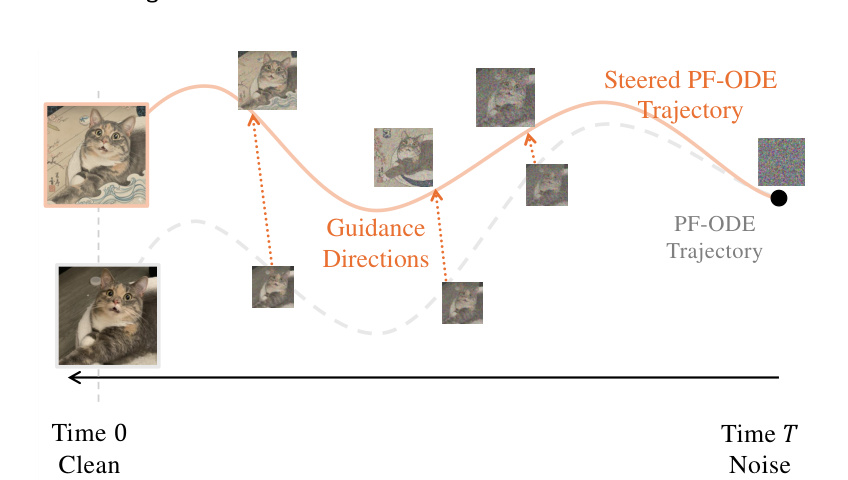
\includegraphics[width=\textwidth,height=0.58\textheight,keepaspectratio]{fig-8-1.jpg}
    \vfill
    \footnotesize
    右（$t=T$，ノイズ）から左（$t=0$，クリーン）へ逆時間PF-ODE。\\
    誘導方向（重み$w_t$）が無条件軌道を属性（例：日本画風）へ曲げる。
\end{frame}
%=============================================
\assuppl
\begin{frame}{\supplmark：図8.1の読み方}
    \begin{columns}[T,onlytextwidth]
        \begin{column}{0.48\textwidth}
            \begin{exampleblock}{灰色：PF-ODE}
                無条件の逆時間軌道。\\
                学習済みスコア場に従う。
            \end{exampleblock}
        \end{column}
        \begin{column}{0.48\textwidth}
            \begin{exampleblock}{橙：誘導付き}
                各時刻の誘導方向が\\
                軌道を望ましい属性へ寄せる。
            \end{exampleblock}
        \end{column}
    \end{columns}
    \vspace{0.35em}
    \begin{block}{要点}
        誘導は「別モデルで一発生成」ではなく、\\
        \textbf{逆時間力学への時間依存な補正}である。
    \end{block}
\end{frame}
%=============================================
\section{原理：ベイズ分解と誘導}
\asmain
\begin{frame}{区切り：原理：ベイズ分解と誘導}
    \tableofcontents[currentsection]
\end{frame}
%=============================================
\asmain
\begin{frame}{条件付きスコアの加法分解}
    各ノイズレベル$t$で、ベイズ則より
    \[
        \nabla_{\vx_t}\log p_t(\vx_t|\bm{c})
        =
        \underbrace{\nabla_{\vx_t}\log p_t(\vx_t)}_{\text{無条件方向}}
        +
        \underbrace{\nabla_{\vx_t}\log p_t(\bm{c}|\vx_t)}_{\text{誘導方向}}
        \tag{8.1.1}
    \]
    \begin{block}{含意}
        真の条件付き逆時間力学は、\\
        無条件スコアに$\nabla_{\vx_t}\log p_t(\bm{c}|\vx_t)$を足せば得られる。
    \end{block}
\end{frame}
%=============================================
\asmain
\begin{frame}{誘導付きPF-ODE}
    正確な条件付きスコアのもとで
    \begin{align*}
        \frac{\mathrm{d}\vx(t)}{\mathrm{d}t}
        &=
        f(t)\vx(t)
        -\frac{1}{2}g^{2}(t)\,
        \nabla_{\vx_t}\log p_t(\vx(t)|\bm{c})
        \tag{8.1.2}
        \\
        &=
        f(t)\vx(t)
        -\frac{1}{2}g^{2}(t)
        \Bigl[
        \nabla_{\vx_t}\log p_t(\vx(t))
        +
        \nabla_{\vx_t}\log p_t(\bm{c}|\vx(t))
        \Bigr].
    \end{align*}
    \begin{itemize}
        \item 正確なスコアと正確な積分なら、$p_T(\cdot|\bm{c})$から$p_0(\cdot|\bm{c})$へ
        \item 標準構成では$p_T(\vx_T|\bm{c})$は条件にほぼ依存しない事前で近似
        \item $\vx$/$\veps$/スコア/$\bm{v}$予測は式6.3.1の線形変換で結べる
    \end{itemize}
\end{frame}
%=============================================
\section{誘導方向の具体化}
\asmain
\begin{frame}{区切り：誘導方向の具体化}
    \tableofcontents[currentsection]
\end{frame}
%=============================================
\asmain
\begin{frame}{三つの入り口（予告）}
    \begin{enumerate}
        \item \textbf{Classifier Guidance（CG，8.2）}\\
        ノイズ時刻の分類器$\nabla_{\vx_t}\log p_\psi(\bm{c}|\vx_t,t)$を直接足す
        \item \textbf{Classifier-Free Guidance（CFG，8.3）}\\
        条件付き・無条件スコアの差として誘導方向を暗に推定
        \item \textbf{学習不要（代理）誘導（8.4）}\\
        タスク損失からの代理ポテンシャルで$G_t$を構成
    \end{enumerate}
\end{frame}
%=============================================
\asmain
\begin{frame}{CG：分類器勾配を足す}
    時刻条件付き分類器$p_\psi(\bm{c}|\vx_t,t)$を\\
    ノイズ付きラベルデータで学習する（Dhariwal \& Nichol, 2021）。
    \[
        \nabla_{\vx_t}\log p_\psi(\bm{c}|\vx_t,t)
        \;\approx\;
        \nabla_{\vx_t}\log p_t(\bm{c}|\vx_t)
    \]
    \begin{block}{サンプリング時}
        この勾配を無条件スコアに加算する。\\
        拡散本体の再学習は不要（分類器は別途）。
    \end{block}
\end{frame}
%=============================================
\asmain
\begin{frame}{CFG：差として誘導を読む}
    単一モデル$s_\phi(\vx_t,t,\bm{c})\approx\nabla_{\vx_t}\log p_t(\vx_t|\bm{c})$を学習し、\\
    条件を特殊なヌルトークンに置き換えて無条件も同時学習する\\
    （Ho \& Salimans, 2021）。
    \begin{exampleblock}{読み替え}
        誘導方向$\nabla\log p_t(\bm{c}|\vx_t)$は、\\
        条件付きスコアと無条件スコアの差として現れる（8.3で展開）。
    \end{exampleblock}
\end{frame}
%=============================================
\asmain
\begin{frame}{学習不要：なぜ代理が必要か}
    標準の前向きノイズでは$\vx_t\sim p_t(\cdot|\vx_0)$で、\\
    前向き核は$\bm{c}$に追加依存しない（$\bm{c}\perp\vx_t\mid\vx_0$）。
    \[
        p_t(\bm{c}|\vx_t)
        =
        \int p(\bm{c}|\vx_0)\,p(\vx_0|\vx_t)\,\mathrm{d}\vx_0
    \]
    \begin{alertblock}{困難}
        この事後平均は一般に計算不能。\\
        $\Rightarrow$タスク固有の代理誘導方向を構成する動機。
    \end{alertblock}
\end{frame}
%=============================================
\asmain
\begin{frame}{損失ベースの代理ポテンシャル}
    オフザシェルフ損失$\ell(\vx_t,\bm{c};t)$（小さいほど条件に合う）から
    \[
        h_t(\vx_t;\bm{c})
        :=
        \exp\bigl(-\tau\,\ell(\vx_t,\bm{c};t)\bigr),
        \qquad \tau>0
    \]
    \[
        G_t(\vx_t,\bm{c})
        :=
        \nabla_{\vx_t}\log h_t(\vx_t;\bm{c})
        =
        -\tau\,\nabla_{\vx_t}\ell(\vx_t,\bm{c};t)
    \]
    \begin{itemize}
        \item CGは$h_t=p_t(\bm{c}|\vx_t)$（実践では$p_\psi$）に対応
        \item 同値な損失：$\ell=-\log p_\psi(\bm{c}|\vx_t,t)$，$\tau=1$
    \end{itemize}
\end{frame}
%=============================================
\section{共通テンプレート}
\asmain
\begin{frame}{区切り：共通テンプレート}
    \tableofcontents[currentsection]
\end{frame}
%=============================================
\asmain
\begin{frame}{誘導付きスコア場}
    正のポテンシャル$h_t$と強度$w_t\ge 0$に対し
    \[
        s^{\mathrm{guide}}(\vx_t,t,\bm{c};w_t)
        :=
        \nabla_{\vx_t}\log p_t(\vx_t)
        +
        w_t\,G_t(\vx_t,\bm{c})
        \tag{8.1.3}
    \]
    \begin{itemize}
        \item 損失ベース：$G_t=-\tau\nabla_{\vx_t}\ell$
        \item 正確なCG：$G_t=\nabla_{\vx_t}\log p_t(\bm{c}|\vx_t)$
        \item CFG：同じ母集団誘導を条件／無条件スコア差で表現
    \end{itemize}
\end{frame}
%=============================================
\asmain
\begin{frame}{傾き密度と固定時刻解釈}
    各固定$t$で、正規化可能なら式(8.1.3)は
    \[
        \tilde{p}^{\mathrm{tilt}}_{t}(\vx_t|\bm{c})
        \;\propto\;
        p_t(\vx_t)\,h_t(\vx_t;\bm{c})^{w_t}
    \]
    のスコア（ベース＝拡散支持、ポテンシャル＝条件へ再重み）。
    \begin{alertblock}{注意}
        $\{\tilde{p}^{\mathrm{tilt}}_{t}\}$は固定時刻の解釈にすぎない。\\
        誘導サンプラの周辺と一致するとは限らず、整合は8.4.2。
    \end{alertblock}
\end{frame}
%=============================================
\section{嗜好整合への橋}
\asmain
\begin{frame}{区切り：嗜好整合への橋}
    \tableofcontents[currentsection]
\end{frame}
%=============================================
\asmain
\begin{frame}{嗜好整合：条件充足だけでは足りない}
    強い制御でも、条件は満たすが好みから外れることがある。
    \[
        \tilde{p}^{\mathrm{tilt}}_{0}(\vx_0|\bm{c})
        \;\propto\;
        p_0(\vx_0|\bm{c})\,
        \exp\bigl(\lambda_{\mathrm{pref}}\,r(\vx_0,\bm{c})\bigr)
    \]
    \begin{itemize}
        \item $r$：嗜好評点、$\lambda_{\mathrm{pref}}>0$（KL正則化では$1/\beta$）
        \item 典型はRLHFだが不安定になりやすい（報酬モデル＋RL）
        \item 8.5：Diffusion-DPOはペア選択から傾きを直接学習
    \end{itemize}
\end{frame}
%=============================================
\section{まとめ}
\asmain
\begin{frame}{区切り：8.1のまとめ}
    \tableofcontents[currentsection]
\end{frame}
%=============================================
\asmain
\begin{frame}{8.1 全体のまとめ}
    \begin{enumerate}
        \item \textbf{動機}
        粗$\to$細の軌道に誘導項を足して意図を反映
        \item \textbf{原理}
        ベイズ分解（8.1.1）と誘導付きPF-ODE（8.1.2）
        \item \textbf{統一形}
        $s^{\mathrm{guide}}=\nabla\log p_t+w_t G_t$（8.1.3）
        \item \textbf{地図}
        CG／CFG／学習不要／嗜好整合（DPO）
        \item \textbf{注意}
        傾き密度は固定時刻解釈；周辺一致は別問題
    \end{enumerate}
\end{frame}
%=============================================
\asmain
\begin{frame}{8.1 全体のまとめ：一本の流れ}
    \begin{block}{今日の道筋}
        制御の動機
        $\;\to\;$
        ベイズ分解
        $\;\to\;$
        誘導テンプレート
        $\;\to\;$
        各手法の予告
    \end{block}
    \begin{block}{核心}
        誘導とは、逆時間スコア場への加法的補正である。\\
        $G_t$の作り方がCG／CFG／代理損失を分ける。
    \end{block}
    \begin{block}{次へ（8.2）}
        Classifier Guidance：分類器勾配とスケール$\omega$。
    \end{block}
\end{frame}
